\chapter{Problems with TS 2.0}
\label{Problems with TS 2.0}
The Trigger Supervisor version 2.x had a few problems that caused
frustrations with both the operators and the developers of the software.

\section{Browser compatibility}
The first and most visible issue is the slow degradation of support for the
interface in modern Web Browsers.

This is due to an effect caused by the movement of major web browser vendors to
become `evergreen`, which started around 2011.

\subsection{Evergreen browsers}
\label{Evergreen browsers}
An evergreen browser, in essence, is a browser that updates itself without the
interaction of the user.
This is the formal definition of an `evergreen` browser, however there are
some new philosophies that come with this approach.

First off, a web browser's version number no longer has a real meaning.
To a user a web browser will now be `versionless`, the user will no longer know
nor care what browser version is running and will actually assume it is the latest
version.
Browser vendors have combined auto-updating with a significant speedup of their
release cycles. Browsers now tend to update their version once a month, rather
than at most once a year (see figure \ref{fig:updateGraph}).

This corresponds to the release early, release often (RERO) software design
philosophy. An approach popular in the open-source community and used for the
development of the Linux kernel\cite{TheCathedralAndTheBazaar}.

\begin{figure}
  \centering
  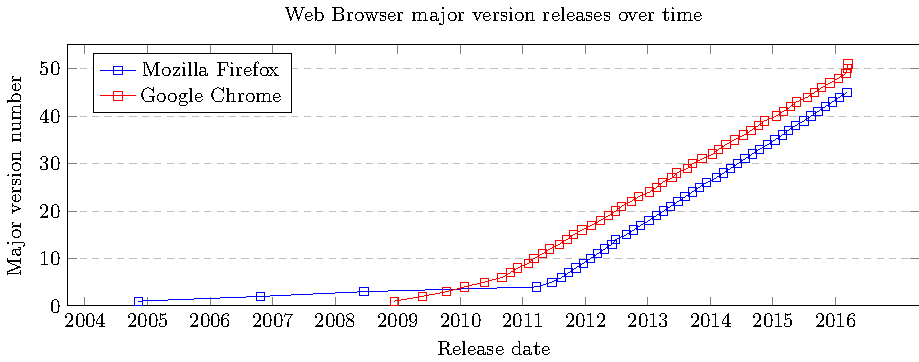
\includegraphics{images/pgfplots/firefox_update_speed-figure0}
  \caption{Overview of major version releases of Mozilla Firefox and Google Chrome over time}
  \label{fig:updateGraph}
\end{figure}

This in turn engaged web browser vendors to implement new standards much faster
and in a much more iterative way than previously possible.
Web browser vendors will no longer develop new features as a whole, but rather
slowly implement a feature piece by piece.
A good example of this is ES6 (sometimes called JavaScript 2015). ES6 is in
essence a set of extra JavaScript functionalities and additions to the syntax.
Without evergreen browsers, this would have been implemented as one big update,
probably in the form of a major release update.
However, evergreen browsers implement every ES6 feature bit by bit. This can be
tracked with the ES6 compat-table project\cite{compattableproject}.

Because of these rapid release cycles and automatic updates, evergreen browsers
introduce a change in behavior of keeping compatibility with older webpages.
If a particular feature would inhibit the development of new features or what is
sometimes referred to as `moving the web forward`, it has become acceptable to
completely remove that feature.
The latest example of this behavior can be found in the rapid implementation,
and equally rapid removal, of the /deep/ and ::shadow CSS selectors\cite{deepAndShadowCSS}.
This goes against the previous philosophy that a web browser must maintain
backwards compatibility with older web pages as much as possible. And this is
the main reason the TS 2.0 interface is experiencing problems with modern browsers.

\subsection{Interface degradation}
\label{Interface degradation}
The age of the TS interface (8 years as of this writing) has reached a point where it
uses HTML, JavaScript, and CSS that is being actively removed by browsers.
This gives some potentially serious issues when operating the interface.

The most prominent example is the modal dialog feature of the interface.
In Mozilla Firefox version 38, the one currently installed in the CMS Control
Room, the modal dialog behaves fine. A white overlay is put over the interface
and a dialog appears, forcing the user to take a decision.
However in the latest version of Firefox, currently 44, the dialog does not appear
while the white overlay does appear. This effectively blocks the user from using
the interface at all from that point and forces a page reload.
Whatever functionality was implemented using the modal dialog is now inaccessible.
See figure \ref{fig:ff38} and \ref{fig:ff44}.
\begin{figure}
  \centering
  \begin{minipage}[b]{0.49\textwidth}
    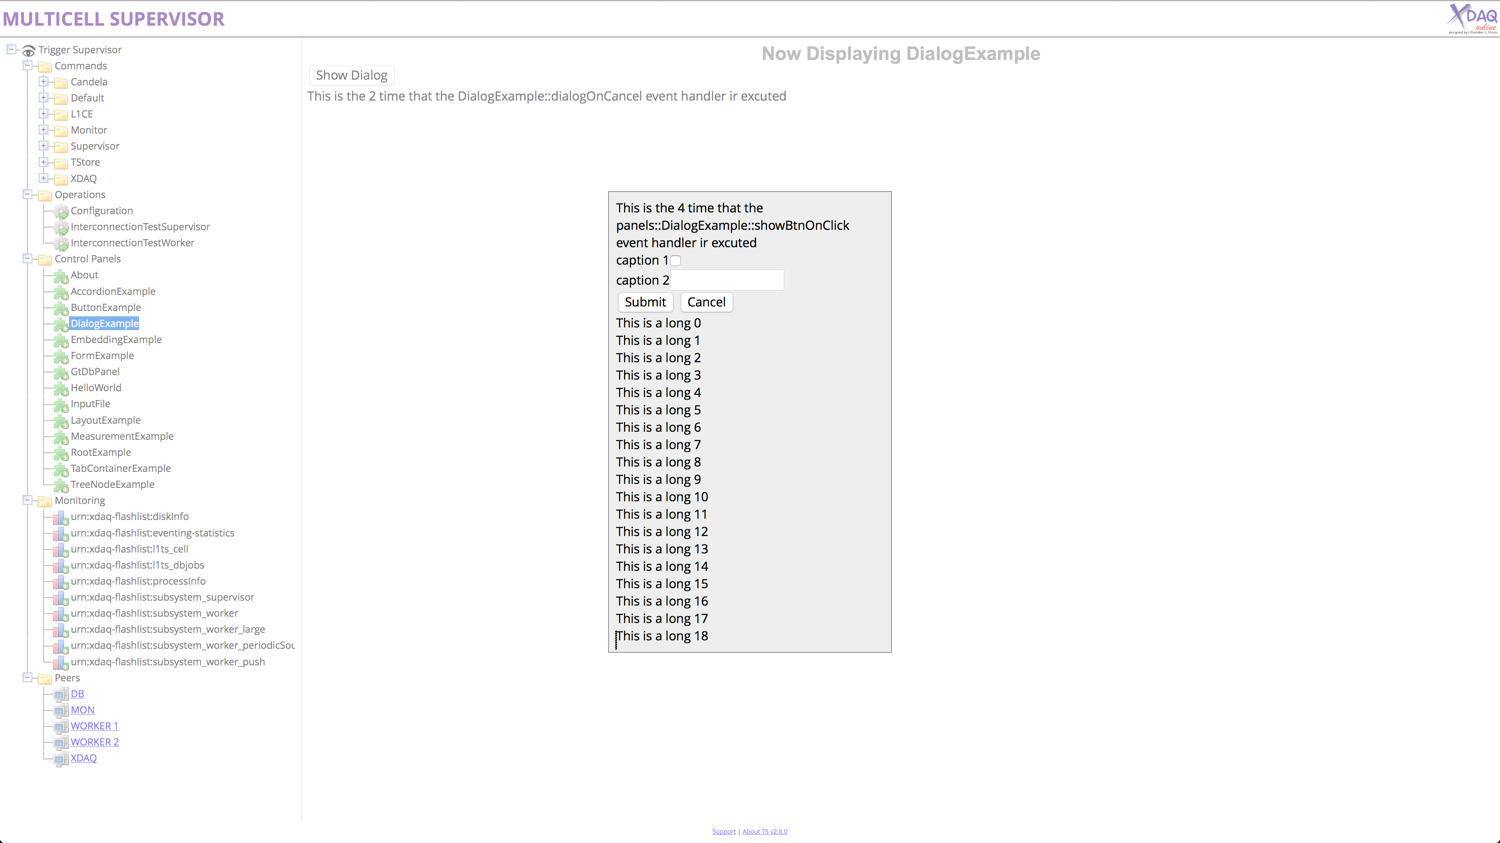
\includegraphics[width=\textwidth]{images/modal_ff38}
    \caption{The modal dialog in Firefox 38}
    \label{fig:ff38}
  \end{minipage}
  \hfill
  \begin{minipage}[b]{0.49\textwidth}
    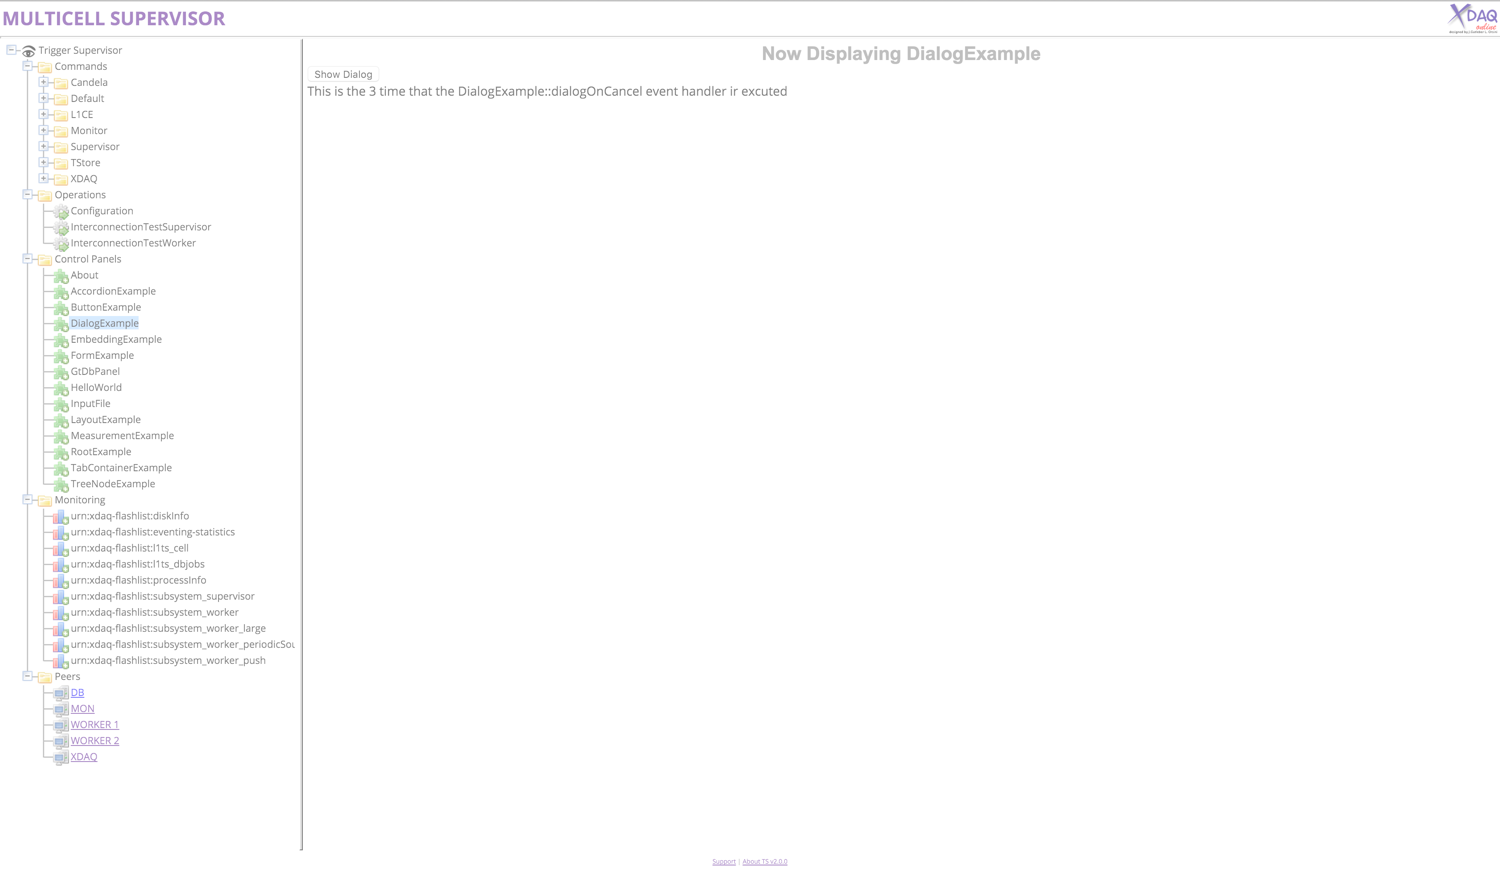
\includegraphics[width=\textwidth]{images/modal_ff44}
    \caption{The modal dialog in Firefox 44}
    \label{fig:ff44}
  \end{minipage}
\end{figure}


\begin{figure}
  \centering
  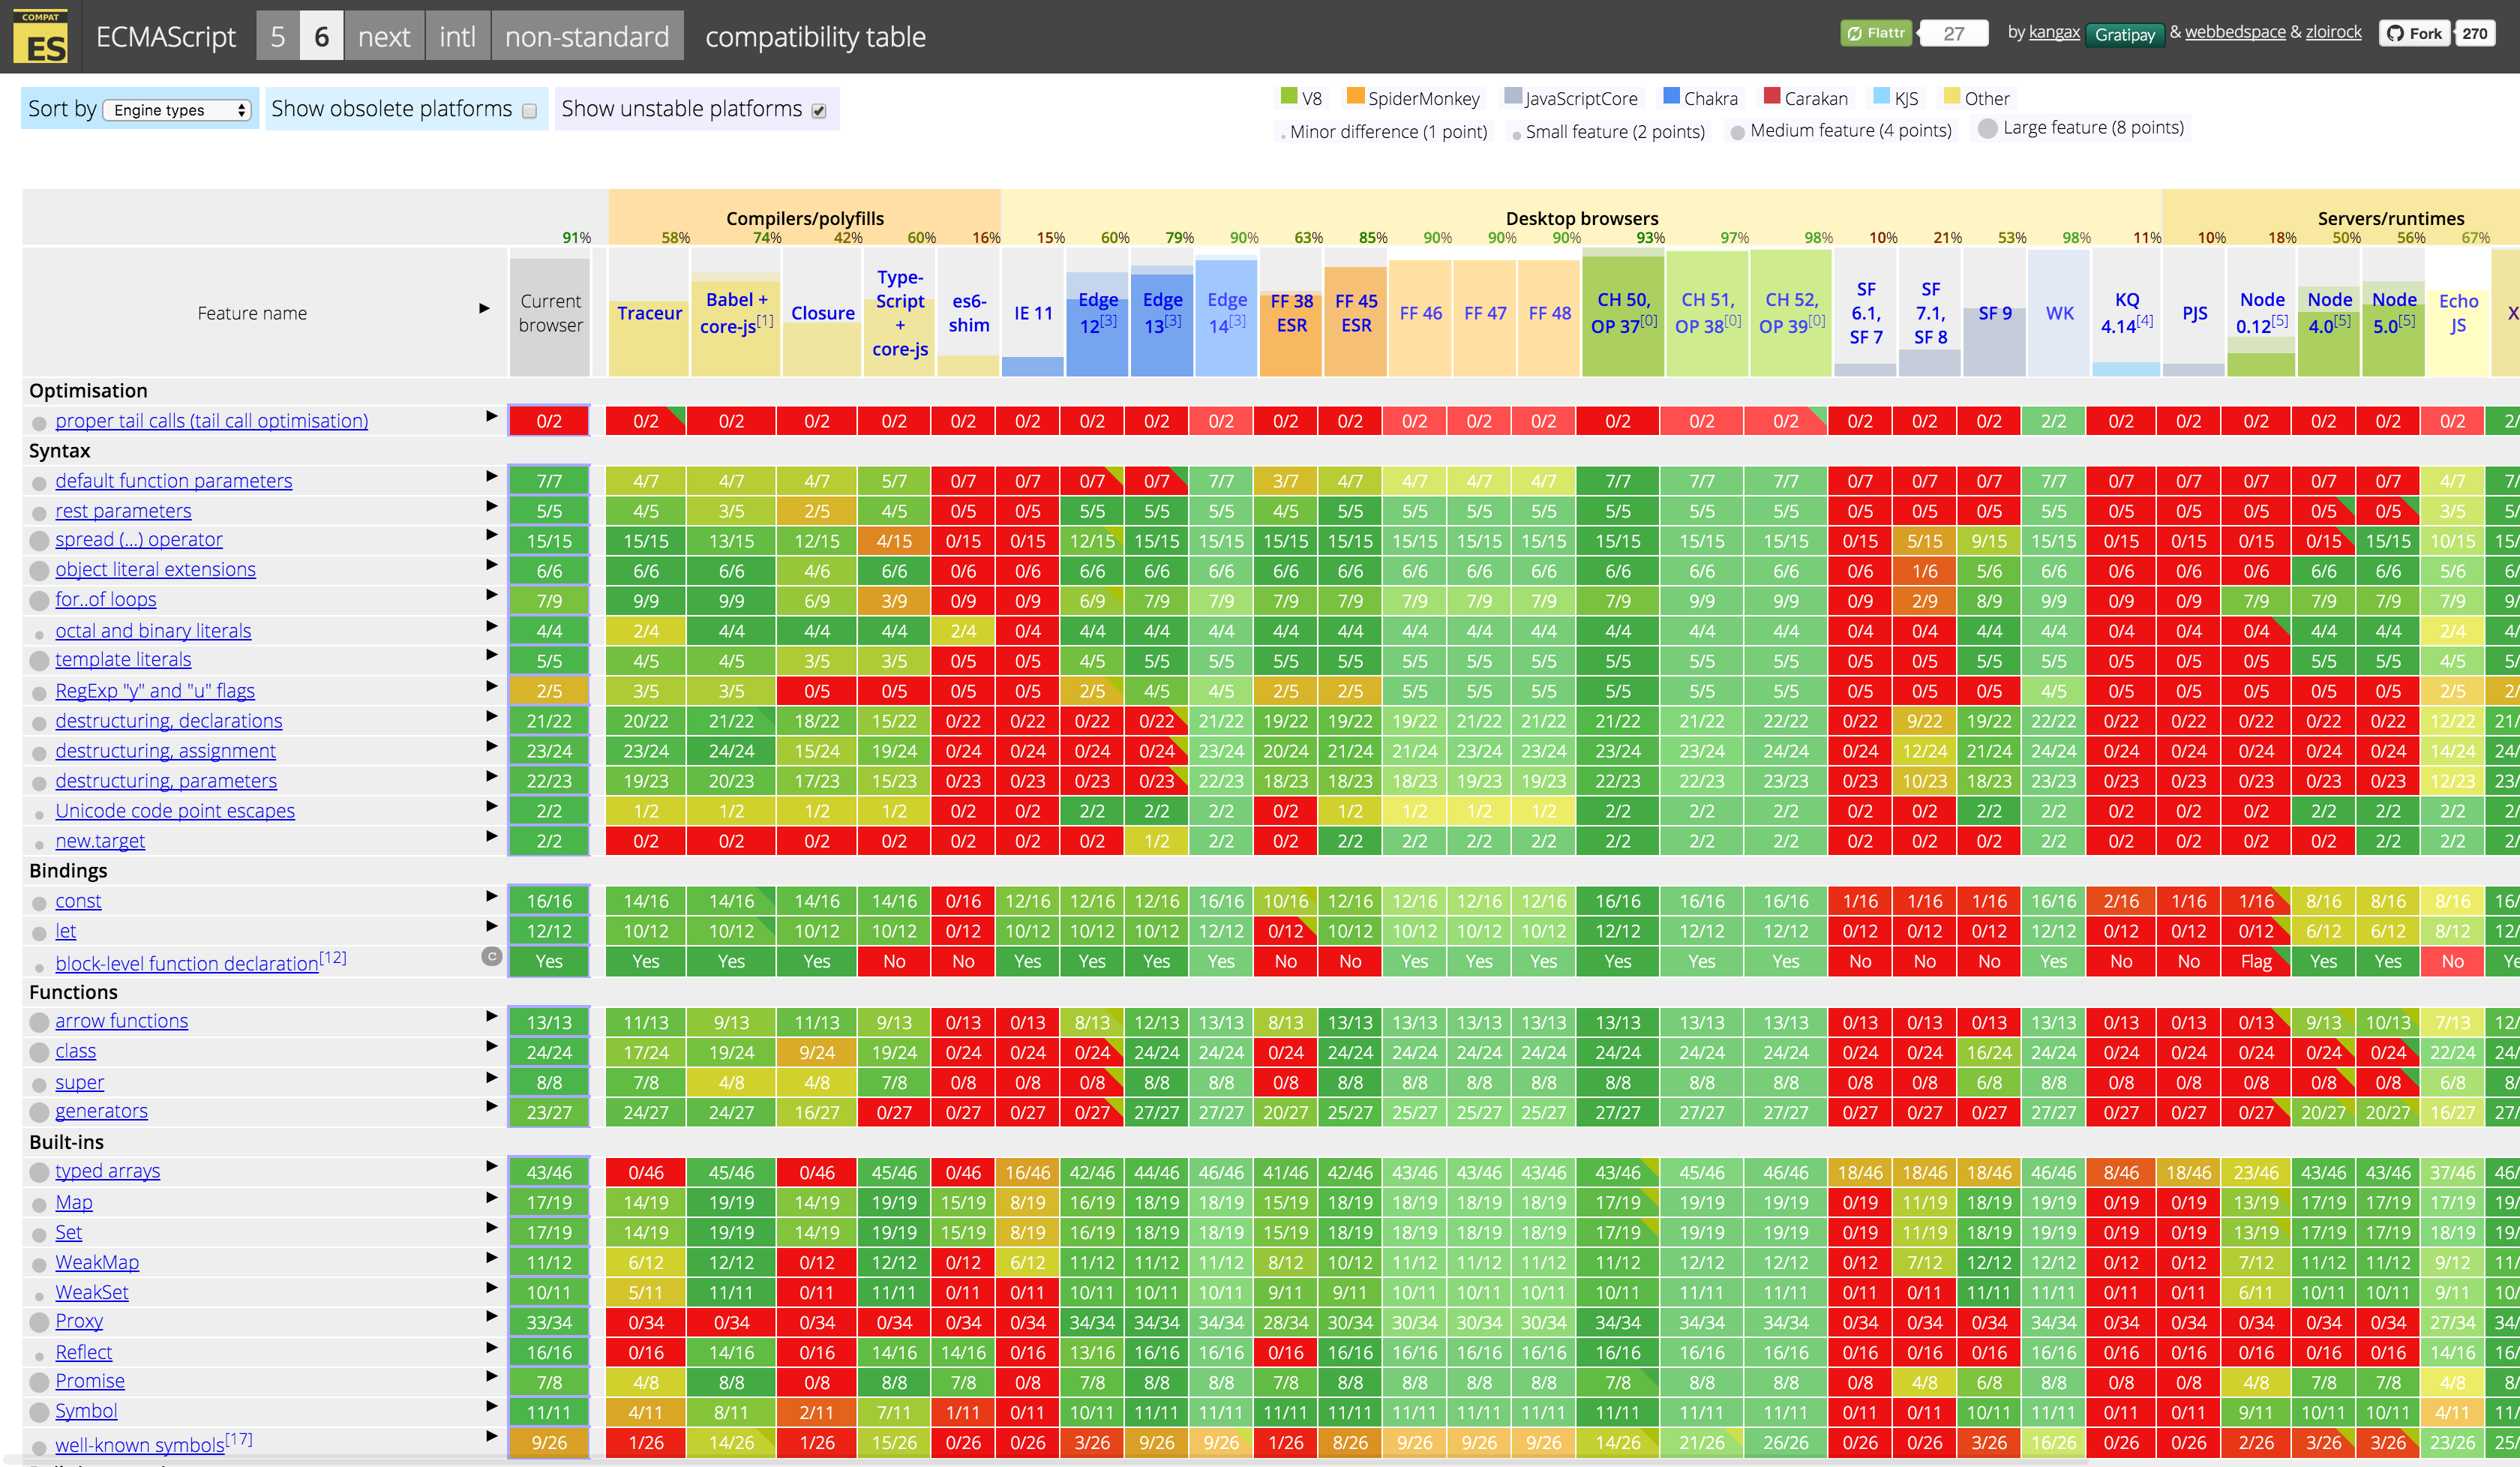
\includegraphics[width=\textwidth]{images/compattable}
  \caption{The ECMAScript compatibility table project}
  \label{fig:compattable}
\end{figure}


CERN uses only Extended Support Releases (ESR) of Firefox, and fortunately in
this case Firefox ESR deployments at CERN are always about a version behind on
the most up-to-date ESR release.
This means the interface degradation is currently not breaking functionality yet,
however it will in the near future and must be addressed as soon as possible.

\subsection{Dojo 0.4}
The front-end JavaScript framework used to render the interface is called Dojo.
It was one of the first JavaScript libraries that successfully attempted to extend
the standard html primitives and one of the few frameworks that worked fully
client-side.

It was very innovative to pick this framework for the first version of the TS.
However, as the version number suggests, it is a beta version. It has some flaws,
one of them being a rather huge memory leak issue (discussed in chapter \ref{Memory-leak problem}),
another being the ever increasing development time when building interfaces with
Dojo 0.4.

\section{Increasing development time}
Dojo 0.4 is around 8 years old now, developed in 2008\cite{TS_PHD}, it cannot be expected to
satisfy modern web application requirements.

It misses helper components to set up a layout, something every modern web
framework has nowadays, and forces the developer to reinvent the wheel
continuously when it comes to interface layouts. This is one of the big reasons
interface code tends to become huge and nigh unreadable.

\fvset{frame=single}
\begin{pyglist}[language=cpp,numbers=left,numbersep=5pt,fontsize=\small]
<!-- A simple title must be coded manually. Prone to typing errors (h2/h4) -->
ajax::PlainHtml* title = new ajax::PlainHtml();
title->getStream() << " <h2 style=\"font-family:arial; color:grey;\"" <<
" align=\"center\">Measurement Example</h4>" << std::endl;
add(title);

<!-- styling must be done manually -->
result_ = new ajax::ResultBox();
result_->setId("subsystem_btnpanel_result_");
result_->set("style","margin:20px; padding:20px; border:2px solid; ");
add(result_);

<!-- some panels need confusing styling to be functional -->
ajax::AccordionContainer* ac = new ajax::AccordionContainer();
ac->set("style","height:80%; width:80%;");
add(ac);
\end{pyglist}
\fvset{frame=none}

It also misses features that cannot be easily compensated. As the requirements
for the Phase II upgrade brings increased complexity, it will translate in the
framework's need to be able to handle increasing amounts of data reliably.
Think for example about large data tables that need filtering and sorting and
manipulation while at the same time keeping memory pressure low.

The current framework simply cannot supply this. And all attempts have resulted
in an ever increasingly slow interface and complexity in use.
For example, an attempt has been made to renew the `operations` interface.
This is an interface that controls a Finite State Machine (FSM) and allows an
operator to direct the flow through this FSM and input configuration parameters
for each transition.
This has been worked on for three months, but was eventually scrapped awaiting
the new TS release and it's new ways to develop interfaces.

\subsection{Maintainability}
The fact that simple tasks take much code to implement, combined with the
ever increasing complexity required from the interface, results in a
maintainability problem. Code becomes unreadable and even small code adjustments
take weeks to implement. Larger tasks or new functionality usually are even more
challenging to implement.

A recent functionality addition that actually made it into release was the ability
to download an arbitrary file from the server.
The requirement was to have a download button next to the text area that already
contained text of the file that would be downloaded.

It took three different approaches to downloading a file, each implementation
more inappropriate than the other. But finally a solution was found, where the file source
is just displayed in a new window, allowing for the user to right-click and
select `download source`.
Any standard or commonly used way to provide downloading of files ended up being
impossible to reliably implement because of the age of the framework TS 2.0
operated on.

This provides another point on why a change was needed.

\subsection{Large input problem}
\label{Large input problem}
The Dojo 0.4 framework uses HTTP GET requests with parameters encoded in the url
to make requests and post data to the cell.
This has some issues one of which recently became a big problem.

First off, HTTP GET, PUT, and DELETE requests should be idempotent. This means
that 2 identical requests at different times must produce identical results.
Not following this principle creates issues when a proxy server is between the
client and the server. A proxy server will always try to cache requests that
are supposed to be idempotent.
Some HTTP headers exist that allow a developer to instruct a proxy server to not cache
a particular request, but it is up to the proxy server implementation to decide
if such a request will be honored, and thus cannot be relied on.

Every request currently has such `no-cache` HTTP headers. And, luckily, no issue with
proxy servers has come up yet, however some browser issues are suspected
to be linked with this issue.

The second issue is the fact that the parameters of every request are url encoded.
This means that parameters are added to the url in the following fashion:
\begin{lstlisting}
http(s)://host:port/path?parameter1=value1&paremeter2=value2
\end{lstlisting}
The problem with this is that there is a maximum length the url is allowed to be,
the exact maximum length depends on both the used browser and server software.

The general consensus is that URLs should be kept under 2KB in size and must not
exceed 8KB, as this is where most browsers and server software draw the line.
Some panels however, like the operations panel, are
designed for very large input variables and far exceeded these limits.

This used to be fine with version 12 of the server software (XDAQ), but in the
recently introduced version 13, a hard limit of 8KB has been introduced.
This breaks important use cases of panels. It is technically possible to change
the Dojo framework's code regarding request handling. However this might
present unforeseen consequences given this is a rather low-level change. Rather
it has been decided TS 2.0 will never run under the new XDAQ 13 version.
